\documentclass[]{article}

\usepackage{fullpage}
\usepackage{amsmath,amsfonts,amsthm,amssymb}
\usepackage{tikz}
\usetikzlibrary{arrows,decorations,patterns,pgfplots.groupplots}
\usepackage{booktabs}


%opening
\title{/r/CFD Challenge 1 - Driven Cavity}

\begin{document}

\maketitle

\section{Objective}

Solve the two-dimensional viscous incompressible Navier-Stokes equations for a shear-driven cavity flow.

\begin{figure}[h]
	\begin{center}
			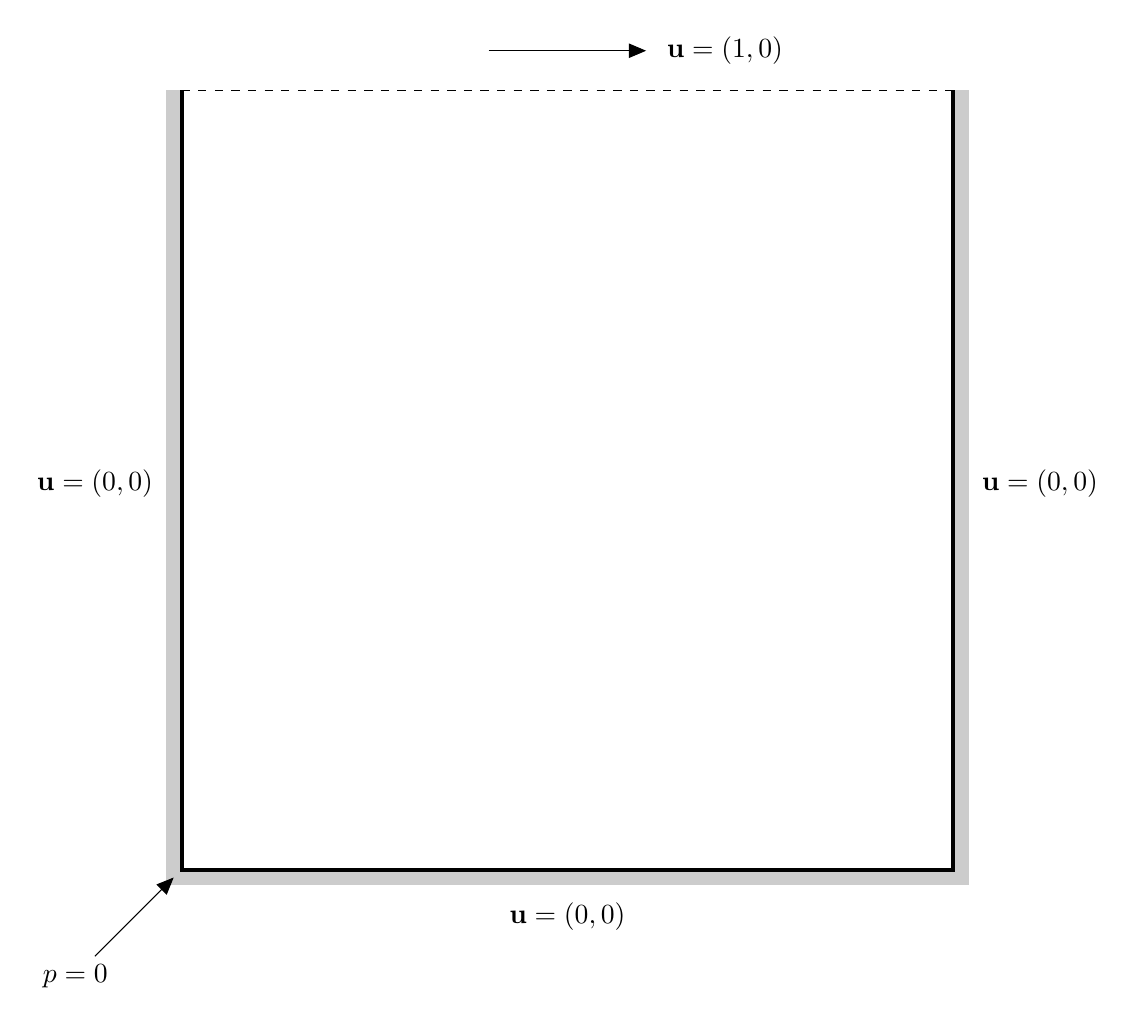
\begin{tikzpicture}[>=triangle 45]
				\draw[line width=2mm,color=gray!40] 
					(0, 0) 
					-- ++ (0,-10) 
					--  ++ (10,0) 
					-- ++ (0,10); 
				\draw[line width=.5mm] (0+1mm, 0) 
					-- ++ (0,-9.9) 
					--  ++ (9.8,0) 
					-- ++ (0,9.9); 

				\draw[dashed] (.1, 0) -- ++(9.8,0);

				\draw[->] (-1,-11) -- (0, -10);
				\path (-1.25,-11.25) node {$p=0$};

				\draw[->] (4,.5) -- (6,.5);
				\path (7,.5) node {$\mathbf{u}=(1,0)$};

				\path (-1,-5) node {$\mathbf{u}=(0,0)$};
				\path (11,-5) node {$\mathbf{u}=(0,0)$};
				\path (5,-10.5) node {$\mathbf{u}=(0,0)$};

			\end{tikzpicture}
		\end{center}
	\caption{Shear-driven cavity flow boundary conditions}
	\label{fig:cavity}
\end{figure}


\section{Governing equations}

The governing equations are the incompressible Navier-Stokes equations, consisting of continuity,
\begin{align}	\label{eq:governing-equations-continuity}
\nabla \cdot \mathbf{u} = {} &  0
\end{align}
and momentum,
\begin{align}	\label{eq:governing-equations-momentum}
\frac{\partial}{\partial t}\left(\textbf{u}\right) + \textbf{u}\cdot\nabla\textbf{u}&=-\nabla p + \frac{1}{Re}\nabla^2\textbf{u}
\end{align}
where non-dimensionalization is by a reference velocity, length, pressure and viscosity,
\begin{align}
p\equiv\frac{p-p_\infty}{\rho U_\infty^2} \\
Re=\frac{U_\infty L}{\nu}.
\end{align}

\section{Boundary conditions}

As shown in figure \ref{fig:cavity}, the lid of the cavity is driven at a non-dimensional velocity of $\mathbf{u}_{\text{lid}} = (1,0)$, while the remaining walls are at rest, $\mathbf{u}_{\text{walls}} = (0,0)$.
The pressure level of the lower left corner is set to zero, $p_{(0,0)}=0$.

\section{Judging}

The submission with the most points will be deemed the winner of this challenge.
Points are awarded for:

\begin{enumerate}
\item \textbf{Reynolds Number}: for the highest resolved Reynolds Number $\log_{10}(Re)$ points will be awarded, so that resolving $Re = 1,000$ awards $3$ points.
Resolving the non-stationary decades below the highest resolved Reynolds number awards an additional point each.
For non-stationary solutions statistically stationary solutions should be used and demonstrated.

\item \textbf{Order of convergence}: the demonstrated spatial and temporal order of convergence is awarded $\max\{0,\log(O)\}+0.5$ points.  
For example, a fourth order spatial convergence rate with a second order temporal convergence will award $2.6$ points.

\item \textbf{CFL limit}: the demonstrated CFL limit is awarded $\max\{0,\log(\text{CFL})\}+0.5$ points.  
For example, a CFL limit of $2.2$ will award $1.3$ points.

\item \textbf{Plots}: up to three points may be earned from plots and animations
	
	\begin{enumerate}
		\item \textbf{Streamline plots}: streamline contour plots for all resolved Reynolds Numbers are worth $0.5$ points if vectorized and $0.25$ points if rasterized.
		
		\item \textbf{Vorticity plots}: vorticity contour plots for all resolved Reynolds Numbers are worth $0.5$ points if vectorized and $0.25$ points if rasterized.
		
		\item \textbf{Velocity profiles}: horizontal and vertical velocity profiles through both the horizontal and vertical lines through the geometric center for all resolved Reynolds Numbers are worth $1$ point if vectorized and $0.5$ point if rasterized.
		
		\item \textbf{Animation}: a time resolved animation from rest to steady state of each of the above is worth $1/3$ of a point.
		
		\item \textbf{Judging}: judges will award up to $3$ points for the quality of the submission.
	\end{enumerate}


\end{enumerate}

A winner for commercial, open-source, and custom codes will be announced along with an overall winner.
Each submission must indicate which category and which code was used.
Each submission must be the original work of the submitter.
The submitter may be anonymous if desired, but should be submitted to /r/CFD.

\end{document}
